%Miriam Clustering
\setlength{\parindent}{0em}
We look for clusters and compare those with the strata. Also we try to observe, if the possibly found clusters have special properties. % Miriam ist doof #truth

%Timo hat fineliner
%oder doch eilaina
In the first step we try to cluster the \textit{Original Data} in \textit{6 Cluster}. Therefore we retrieve the original data set in RapidMiner and choose k as 6.
 
\begin{figure}[!htbp]
\vspace*{-1.5em}
\centering
\begin{subfigure}{.35\textwidth}
  \centering
  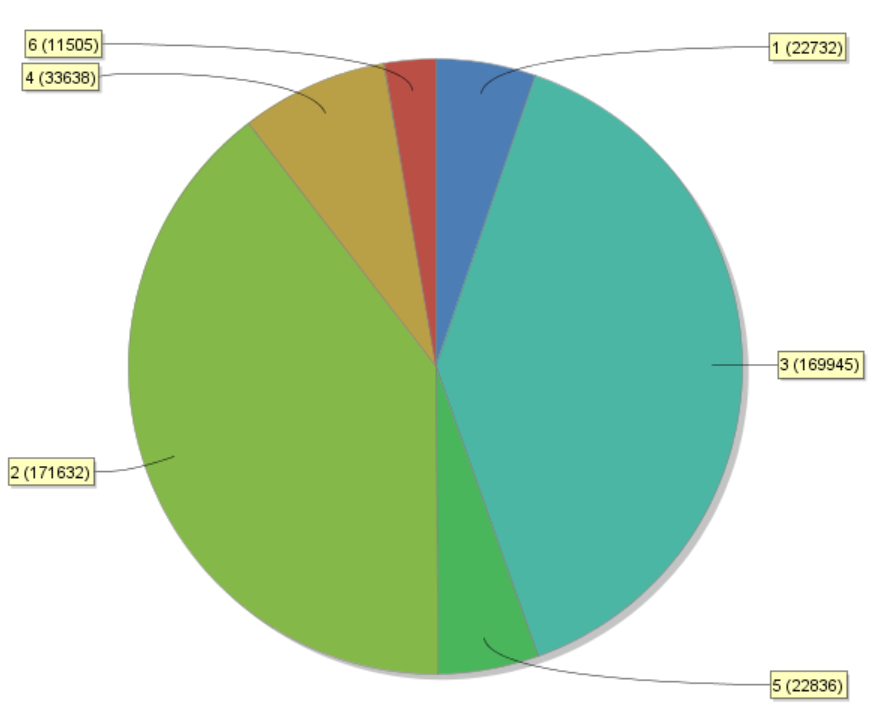
\includegraphics[width=.8\linewidth]{ClusterOrigRapidStrata.PNG}
  \caption{Strata}
  \label{fig:OrgSt}
\end{subfigure}%
\begin{subfigure}{.35\textwidth}
  \centering
  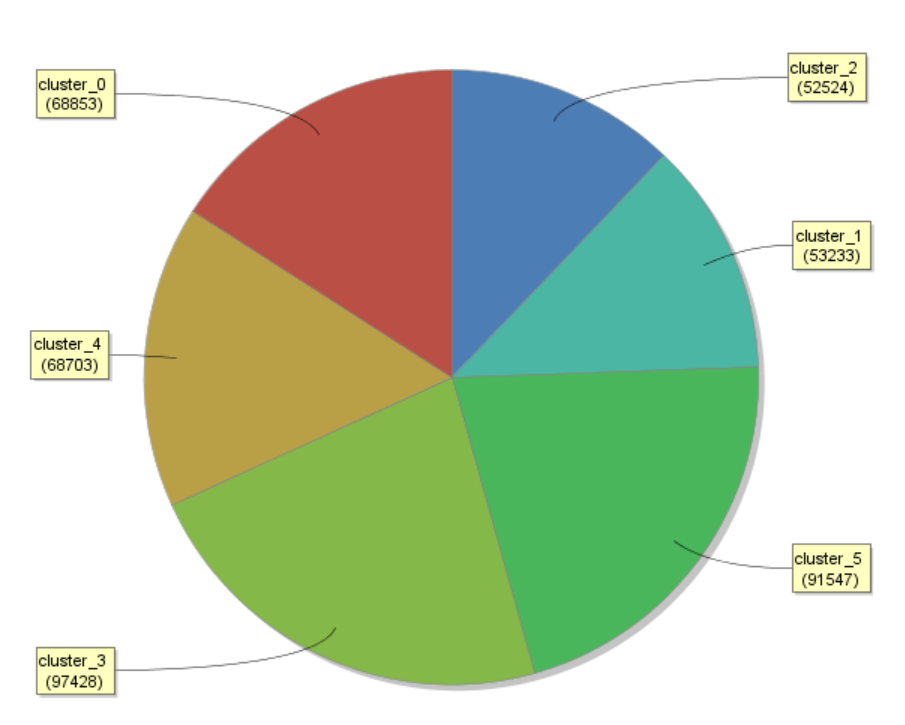
\includegraphics[width=.8\linewidth]{ClusterOrigRapidCluster.PNG}
  \caption{Cluster}
  \label{fig:OrgCl}
\end{subfigure}
\caption{Distribution of original data}
\label{fig:OrgDist}
\end{figure}
\vspace*{-1.5em}

In \Cref{fig:OrgDist} is the result to see of the first try. \Cref{fig:OrgSt} shows the strata distribution as pie chart and \Cref{fig:OrgCl} the resulted cluster distribution. It can already been seen, that the distributions are not similar. For more steps the outcome is analogous.

The next idea is: are 6 cluster too fine? Based on the grouped strata we look at 3 clusters.

\begin{figure}[H]
\centering
\begin{subfigure}{.4\textwidth}
  \centering
  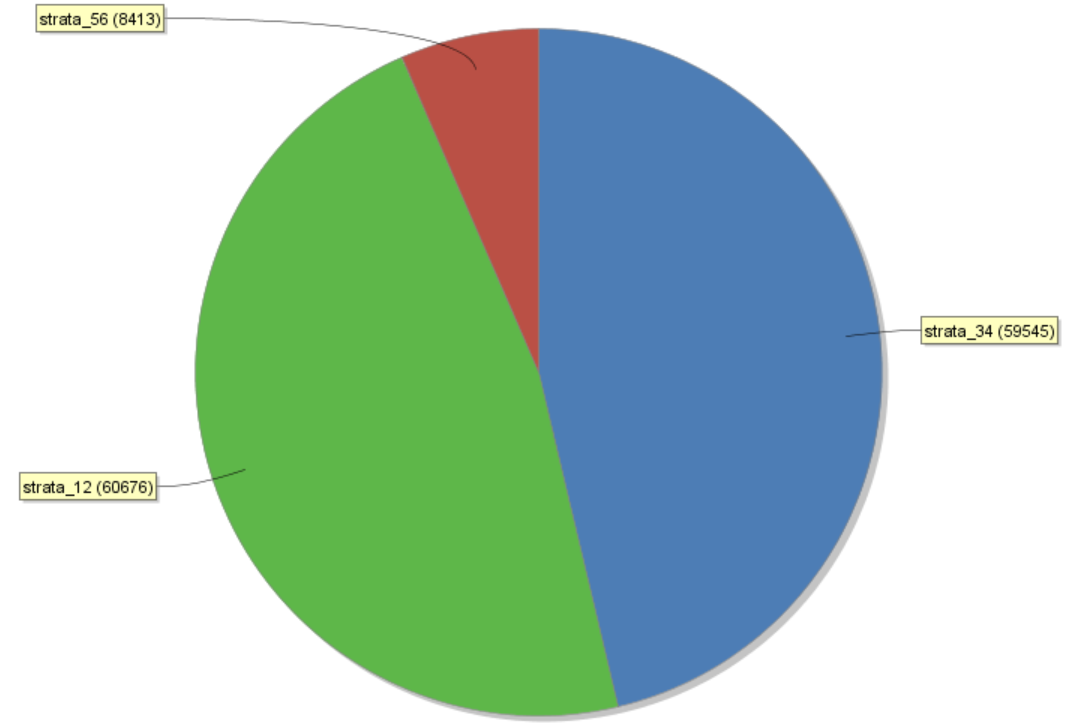
\includegraphics[width=.8\linewidth]{ClusterOrigRapidStrata2Cluster.PNG}
  \caption{Strata}
  \label{fig:OrgSt3}
\end{subfigure}%
\begin{subfigure}{.35\textwidth}
  \centering
  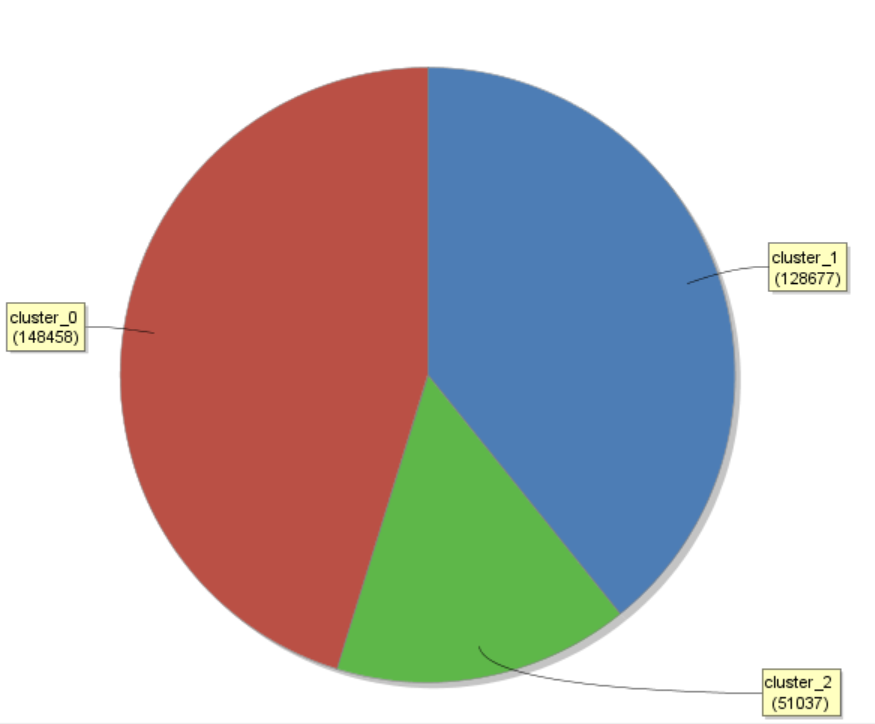
\includegraphics[width=.8\linewidth]{ClusterOrigRapidCluster2Cluster.PNG}
  \caption{Cluster}
  \label{fig:OrgCl3}
\end{subfigure}
\caption{Distribution of original data for just 3 clusters}
\label{fig:OrgDist3Cl}
\end{figure}

\begin{figure}[!htbp]
\centering
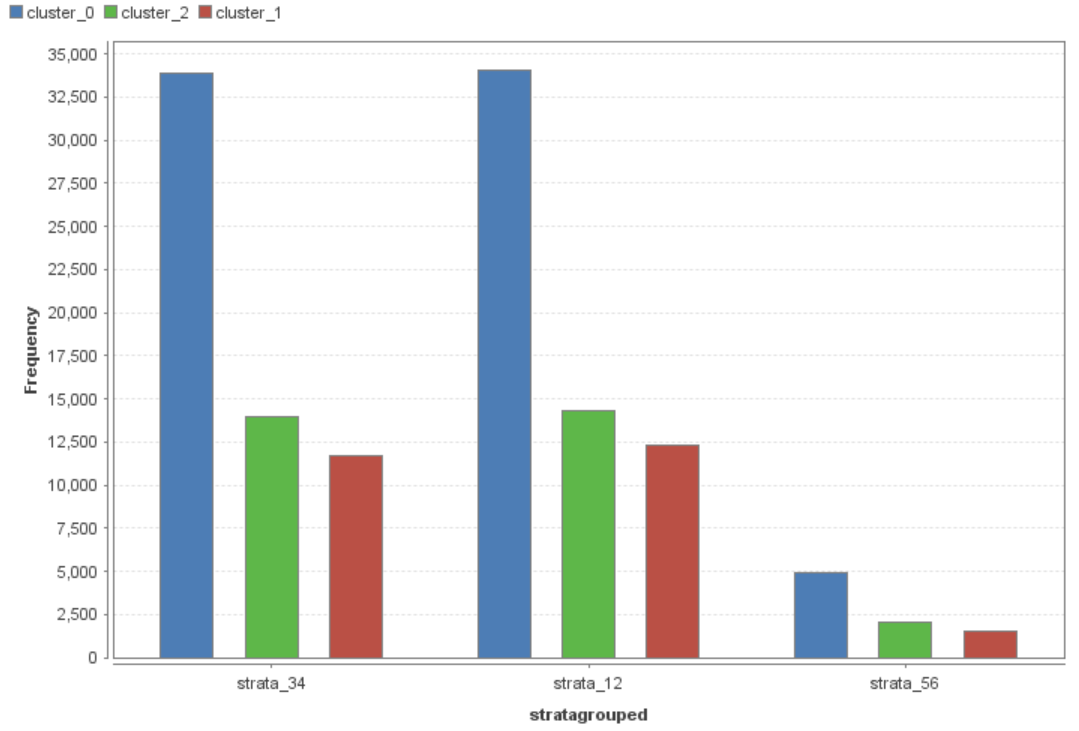
\includegraphics[width=0.5\textwidth]{ClusterOrigRapidDistribution2Cluster.PNG}
\caption{Distribution of the clusters in between the grouped strata}
\label{fig:Groupdist}
\end{figure}
%#ArschFuerNachbarn
%#BloederKommentar
%#0:15

\Cref{fig:OrgDist3Cl} looks promising, so we had a look at the cluster distribution in the 3 grouped stratas, visualized \Cref{fig:Groupdist}. It can be seen, that all clusters appear in all grouped strata. 

\begin{figure}[!htbp]
\vspace{-3em}
\centering
\begin{subfigure}{0.45\textwidth}
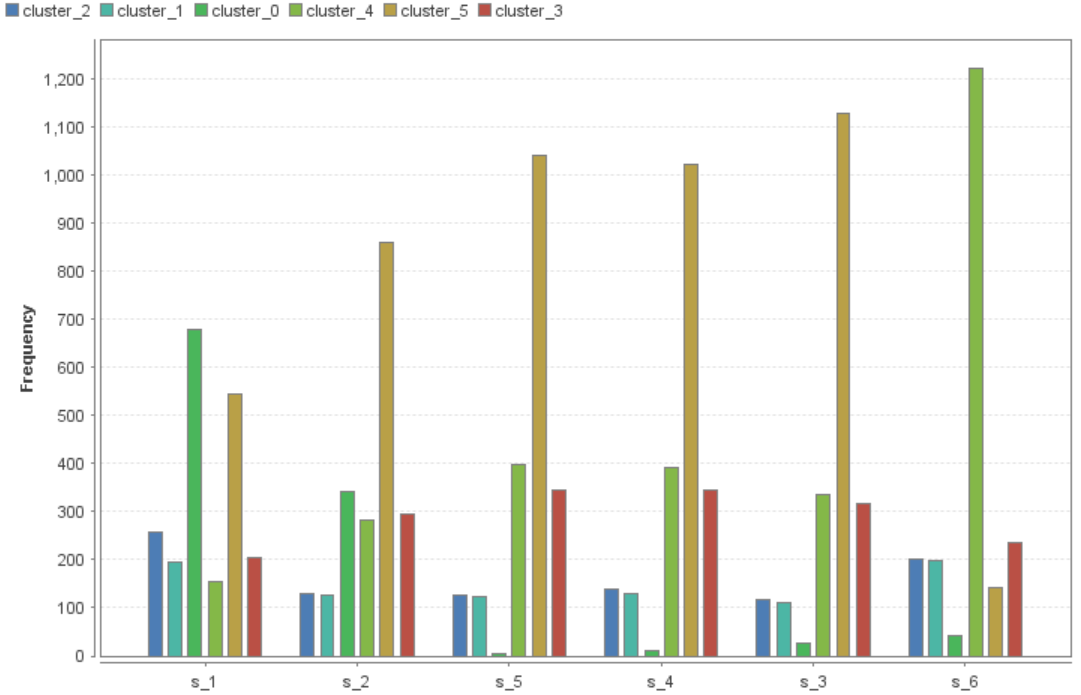
\includegraphics[width=\linewidth]{ClusterOrigRapidDistribution2038eq.PNG}
\caption{For 6 clusters}
\label{fig:2038_6}
\end{subfigure}
\begin{subfigure}{0.45\textwidth}
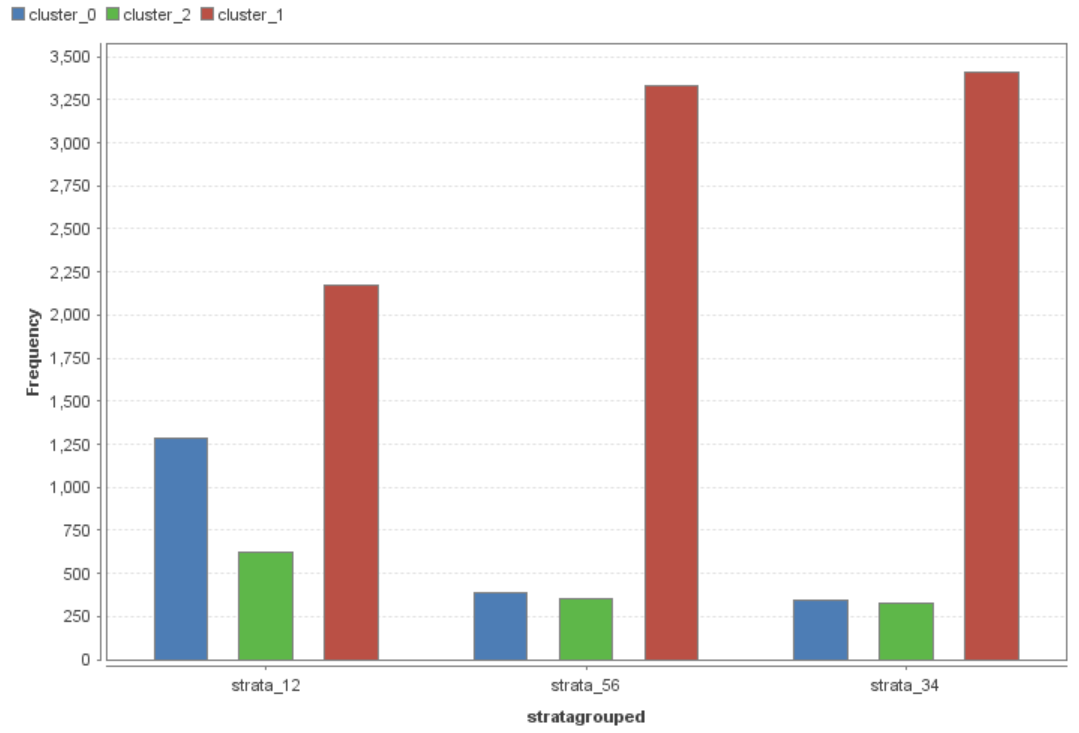
\includegraphics[width=\linewidth]{ClusterOrigRapidDistribution2038eq2.PNG}
\caption{For 3 clusters}
\label{fig:2038_3}
\end{subfigure}
\caption{Distribution of the clusters in between the strata dataset size 2038}
\label{fig:2038_Clust}
\vspace{-3em}
\end{figure}
\vspace{-3em}
\begin{figure}[H]
	\vspace{-3em}
	\centering
	\begin{subfigure}{.43\textwidth}
		\centering
		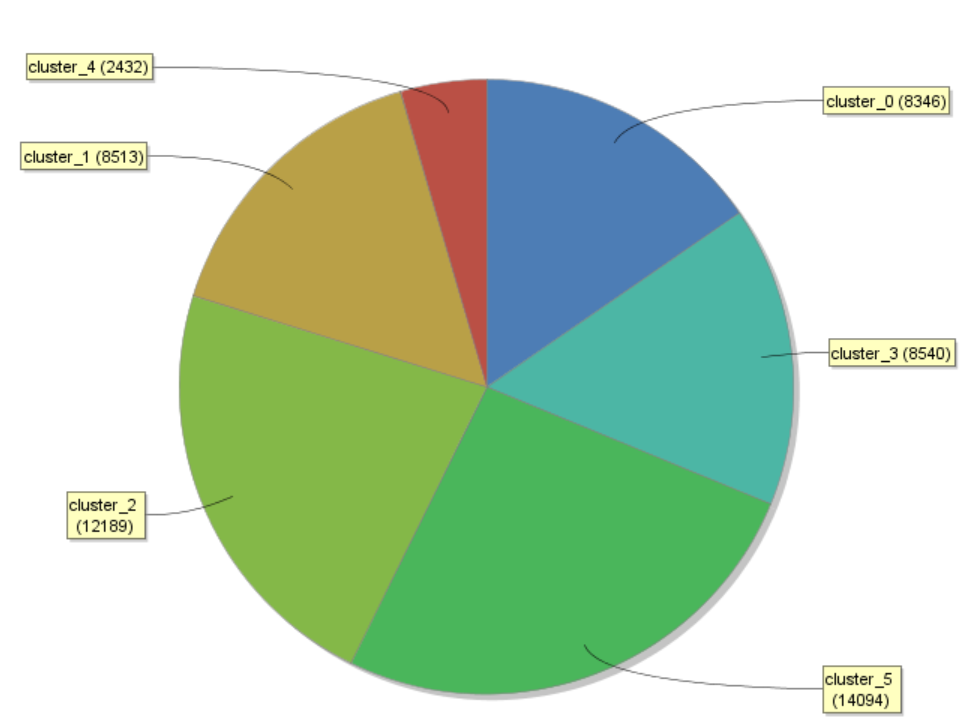
\includegraphics[width=.9\linewidth]{vectorclusteringcluster.PNG}
		\caption{Strata}
		\label{fig:VecSt}
	\end{subfigure}%
	\begin{subfigure}{.4\textwidth}
		\centering
		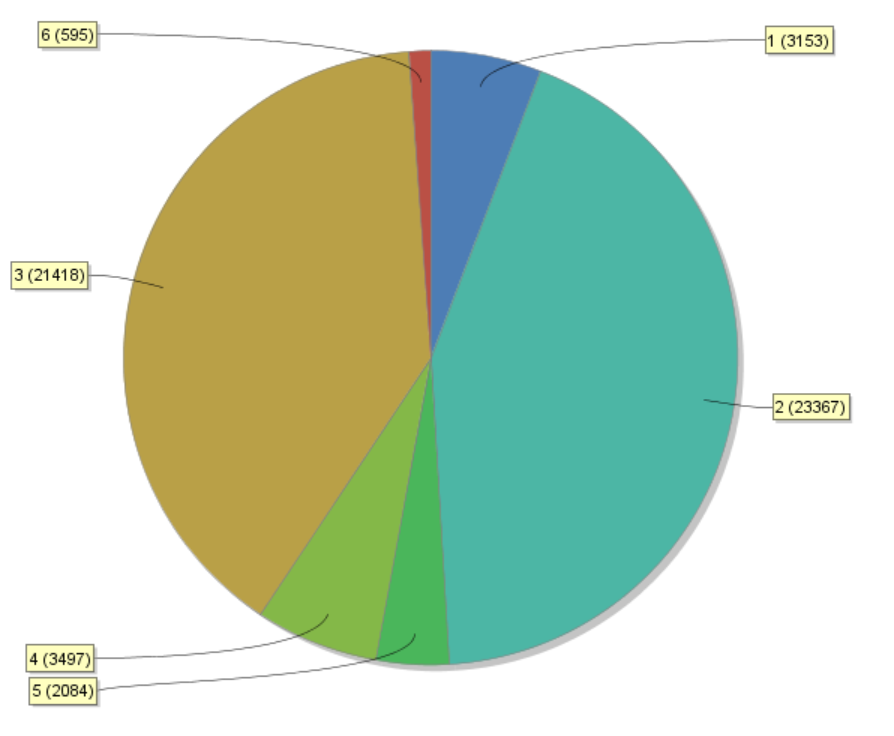
\includegraphics[width=.9\linewidth]{vectorclusteringstrata.PNG}
		\caption{Cluster}
		\label{fig:VecCl}
	\end{subfigure}
	\caption{Distribution of stratified person data}
	\label{fig:VecDist}
\end{figure}

\begin{figure}[H]
	\centering
	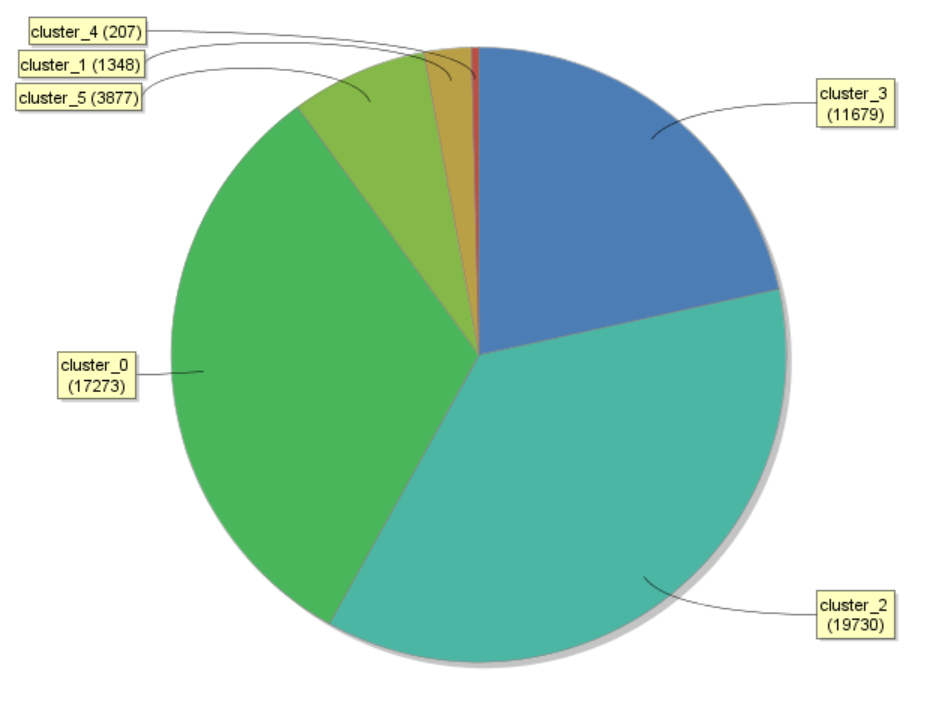
\includegraphics[width=0.4\textwidth]{vectorclusteringcluster1000.PNG}
	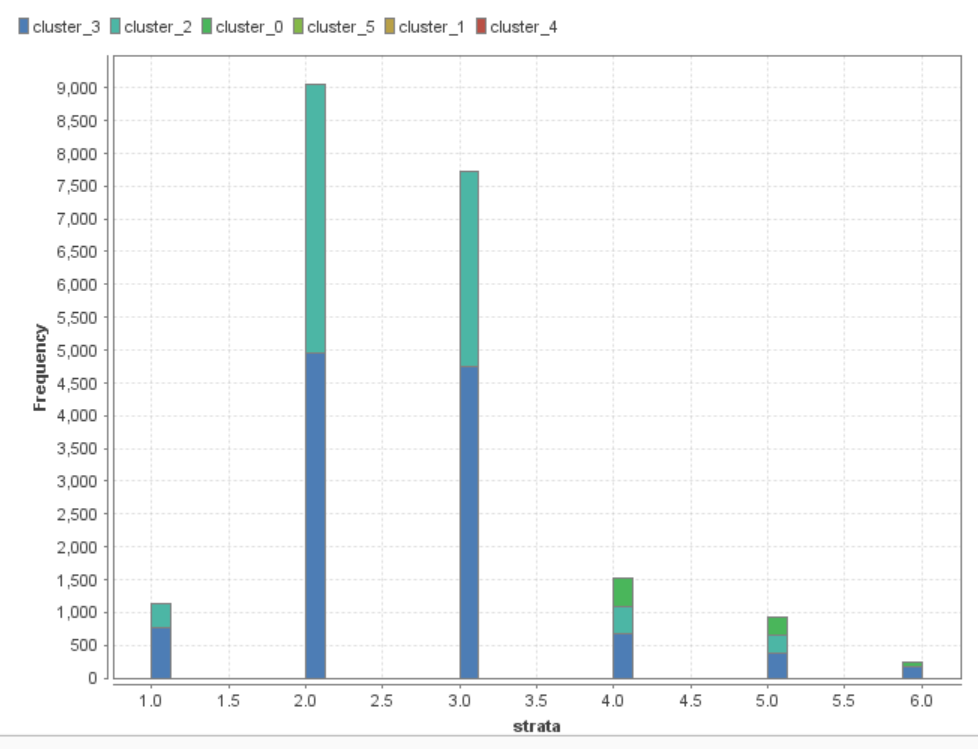
\includegraphics[width=0.49\textwidth]{vectorClustering1000.PNG}
	\caption{1000 steps clustering in 6 clusters on maximal stratified person dataset}
	\label{fig:1000vect}
\end{figure}

Different dataset sizes and equal distribution of the stratas do not effect the result. In  \Cref{fig:2038_Clust} two clustering results can be seen. Again we could not observe a significant correlation.

After those not convincing results we applied the process to the \textit{stratified person data}.



The results for the whole data set without equalization are shown in \Cref{fig:2038_Clust}. We change the number of steps to 1000 for comparison and the result, illustrated in \Cref{fig:1000vect}, lets us assume, that 3 clusters would fit better. 


\begin{figure}[H]
\centering
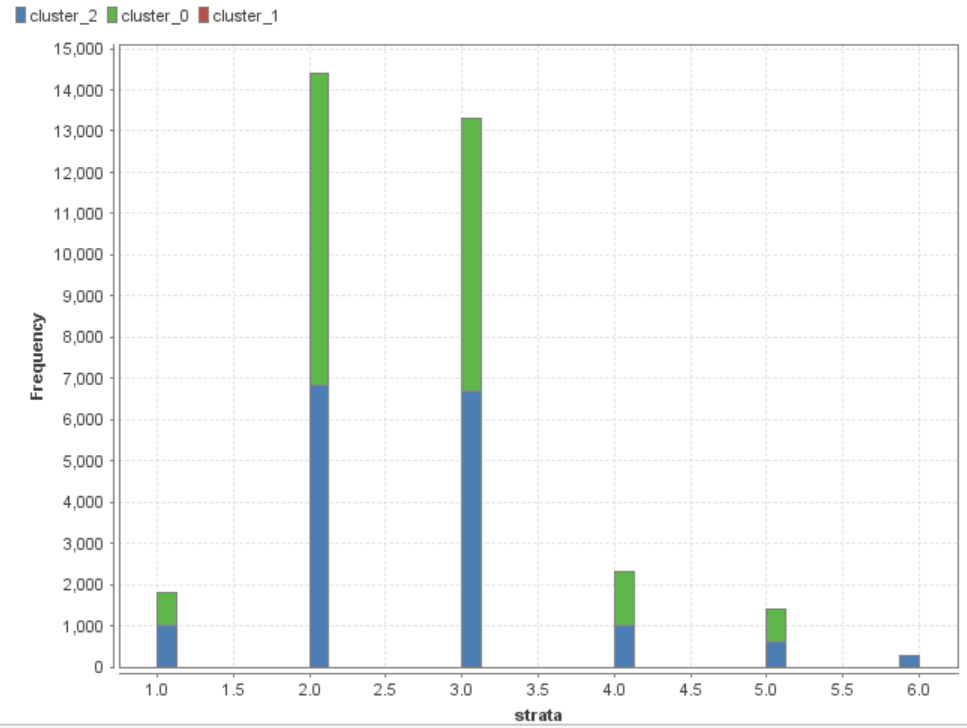
\includegraphics[width=0.69\textwidth]{vectorClustering31000.PNG}
\caption{1000 steps clustering in 3 clusters on maximal stratified person dataset}
\label{fig:1000vect3}
\end{figure}

\Cref{fig:1000vect3} shows clearly, that again no correlation can be found. Applying the procedure to the different datasets we generated creates similar results.


%PCA?

As an improvent of time behaviour and as a further we apply the PCA process on the \textit{original data} without strata and a variance
threshold of 0.95. We get two Attributes, so we can assume, that the data is strongly corrleated. As expected the computating time decreases a lot for the whole process of clustering. 


\begin{figure}[H]
\vspace*{-1em}
\centering
\begin{subfigure}{.3\textwidth}
  \centering
  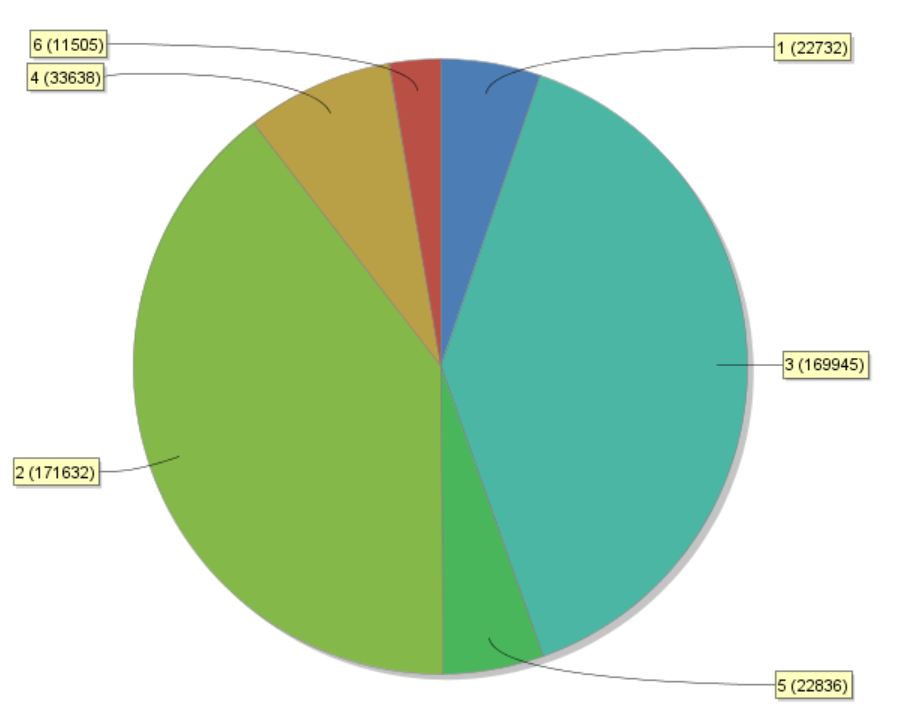
\includegraphics[width=.9\linewidth]{ClusterPCAOrigRapidStrata.PNG}
  \caption{Strata}
  \label{fig:PCAOrgSt}
\end{subfigure}%
\begin{subfigure}{.3\textwidth}
  \centering
  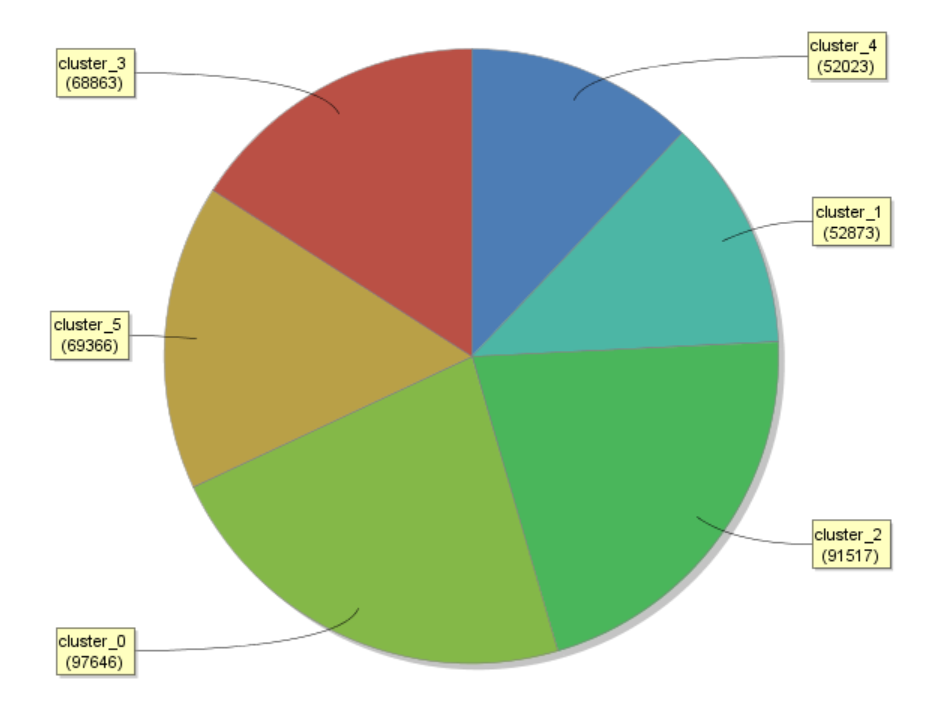
\includegraphics[width=.9\linewidth]{ClusterPCAOrigRapidCluster.PNG}
  \caption{Cluster}
  \label{fig:PCAOrgCl}
\end{subfigure}
\begin{subfigure}{.3\textwidth}
  \centering
  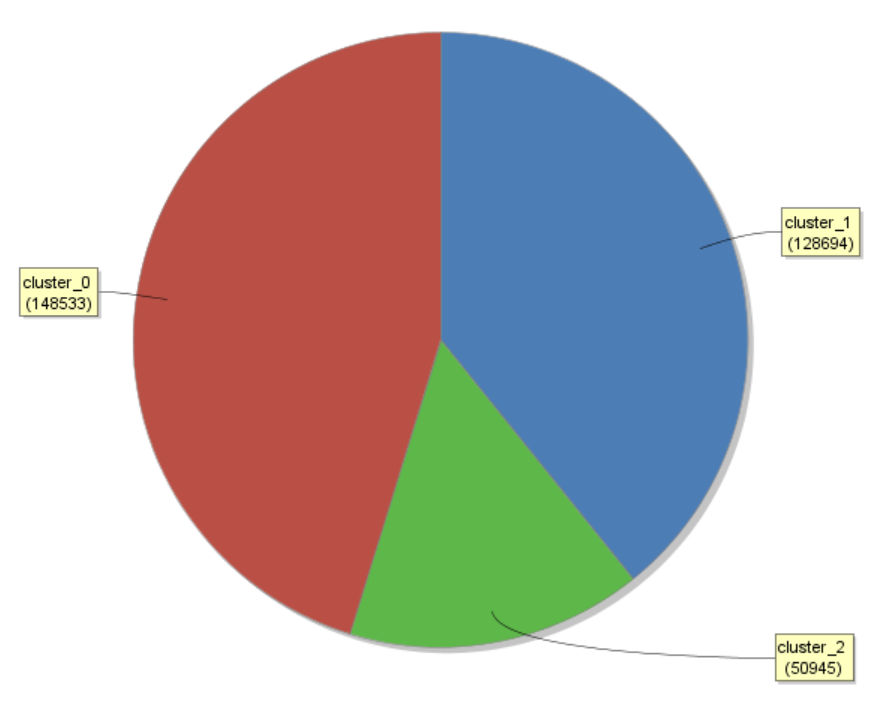
\includegraphics[width=.9\linewidth]{ClusterPCAOrigRapidCluster2Cluster.PNG}
  \caption{3Cluster}
  \label{fig:PCAOrgCl3}
\end{subfigure}
\caption{Distribution of original data}
\label{fig:PCAOrgDist}
\vspace*{-2em}
\end{figure}

For a clustering of 6 clusters we get a distribution, which can be seen in \Cref{fig:PCAOrgDist}, similar to the one we got from the k-means process with the same comfigurations. 
For a clustering of 3 clusters we get again results, that are not clear, visible in \Cref{fig:PCAOrgCl3}.


Using different dataset results in comparable unrewarding result.
\vspace*{-2em}